\section{Cloud Computing}
 A continuación se presentan las definiciones de algunos conceptos importantes relacionados a cloud computing.
\begin{itemize}
\item Cloud : En cloud computing, la palabra cloud o nube es usado como metáfora para “internet”. 
\item Multitenencia : Es una sola instancia de software que corre en la infraestructura del proveedor y sirve a múltiples organizaciones de clientes. Este modelo se diferencia de las arquitecturas con múltiples instancias donde cada organización o cliente tiene su propia instancia instalada de la aplicación. 
\item Despliegue : Despliegue. Un despliegue de servicios es una instancia de un servicio alojado en el cloud, ya sea en un ambiente de pruebas, en un entorno de producción, o en ambos.
\item Datacenter : Un datacenter es un edificio o sala de gran tamaño usada para mantener en él una gran cantidad de equipamiento electrónico. Suelen ser creados y mantenidos por grandes organizaciones con objeto de tener acceso a la información necesaria para sus operaciones.
\item SOA : Es un paradigma de arquitectura para diseñar y desarrollar sistemas distribuidos. Las soluciones  SOA  han sido creadas para satisfacer los objetivos de negocio las cuales incluyen facilidad y flexibilidad de integración con otros sistemas, alineación directa a los procesos de negocio reduciendo costos de implementación, innovación de servicios a clientes y una adaptación ágil ante cambios incluyendo reacción temprana ante la competitividad.
\item Escalabilidad : Un sistema informático es escalable si puede crecer para responder ante necesidades mas exigentes. 
\item Elasticidad: La elasticidad consiste en la potencia de escalar los 
recursos informáticos ampliándolos y reduciéndolos con una fricción mínima. 
\end{itemize}


\section{Introducción}
Cloud computing, también llamado computación en la nube o servicios en la nube, es un paradigma que permite ofrecer servicios de computación a través de internet. Dichos servicios pueden ser por ejemplo redes, servidores, almacenamiento, aplicaciones.

Es un nuevo modelo de prestación de servicios de negocio y tecnología que permite al usuario acceder a un catálogo de servicios estandarizados y responder con ellos las necesidades de negocio, en forma flexible y adaptativa. 
Permite aumentar el número de servicios basados en la red, esto genera beneficios tanto para los proveedores que pueden ofrecer de forma mas rápida y eficiente un mayor numero de servicios como para los usuarios que tienen la posibilidad de acceder a ellos. El acceso a los recursos es totalmente transparente e inmediato y mediante un modelo de pago por consumo, brindándole al usuario la sensación de poseer infinitos recursos.
\section{Modelos de Servicios}
Existen tres modelos de servicios que se pueden ver como capas sobre las cuales podían construirse y desplegarse aplicaciones distribuidas. Estas capas son infraestructura, plataforma y software.
En la figura (\ref{fig:Modelo_servicios})
podemos observar los distintos modelos y los respectivos controles de usuario y proveedor. 

\begin{figure}[!ht]
\centering
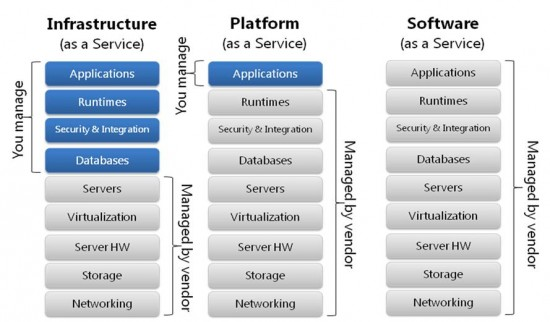
\includegraphics[width=\columnwidth, keepaspectratio]{_imagenes/Modelo_servicios.jpg}
\caption{Mar Atlántico.} \label{fig:Modelo_servicios}
\end{figure}

\begin{description}
\item[Cloud Software as a Service (SaaS).] El servicio provisto al usuario consiste en consumir una aplicación que es ejecutada en la nube, a demanda, vía multitenencia. Las aplicaciones que suministran este modelo de servicios son accedidas mediante un navegador web o de cualquier aplicación diseñada para tal efecto.  
El usuario no tiene control sobre la infraestructura de la nube, siendo transparente para el y eliminando la necesidad de instalar la aplicación en sus propias computadoras evitando costes de hardware y mantenimiento.  

\item[Cloud Platform as a Service (PaaS).] El servicio provisto al usuario consiste en utilizar la infraestructura de la nube para ejecutar aplicaciones desarrolladas por el usuario o adquiridas a terceros. 
Es la encapsulación de una abstracción del ambiente de desarrollo con sus modelos.  
El usuario no maneja ni controla la infraestructura de la nube, pero tiene control sobre la aplicación que es ejecutada y también sobre la configuración de entorno de ejecución de la aplicación. 

\item[Cloud Infraestructure as a Service (IaaS).] El servicio provisto al usuario consiste en la infraestructura de ejecución. El usuario es capaz de ejecutar código arbitrario, controla el sistema operativo y todas las aplicaciones de la nube. 
El hardware está virtualizado en la nube y se provee al usuario recursos como servidores, almacenamiento, redes, etc. Cada vez es mas adoptado este modelo, sobre todo por una gran cantidad de startups que lo utilizan por no poder permitirse tener datacenters propios. Provee mecanismos fáciles para que los desarrolladores interactúen con el IaaS generalmente creando maquinas virtuales. La interacción de las aplicaciones con IaaS suele ser a través de SOA con contratos de servicios, mediante WSDL o REST.
Está dirigido a empresas que desean delegar la implantación de sus sistemas  en la infraestructura hardware de un proveedor externo, o servicios de almacenamiento externo, copias de seguridad de sus datos, cálculos complejos que requieran software de elevadas prestaciones, entre otros. El proveedor les permitirá gestionar dichos sistemas en un entorno virtualizado. 

\end{description}

\section{Modelos despliegue}

Existen tren modelos de despliegue o tipos de cloud, el tipo de cloud a adoptar se debe definir en base a quien va a poder acceder a los servicios y a quien va a gestionar la infraestructura. Los tipos son privadas, públicas e híbridas y a continuación se explican cada una de ellas.

\begin{description}
\item[Cloud privado] Una nube privada es aquella en la que solamente una organización, utilizando tecnologías como virtualización, tiene acceso a los recursos que se utilizan para implementar en la nube. Podría compararse con los datacenter que disponen algunas empresas, con infraestructura y máquinas propias dimensionadas en base a la demanda esperada. Mediante la virtualización se puede añadir a las características de los datacenters los beneficios del cloud como la agilidad de provisión o cierto nivel de elasticidad. 
La principal ventaja es que generan seguridad para los clientes ya que no comparten recursos con otros usuarios. La capacidad de elegir el proveddor permite a los clientes seleccionar los recursos tecnológicos que se mejor se adapten a sus necesidades técnicas y económicas.
La desventaja que presenta este modelo es que al ser infraestructuras dedicadas al autoconsumo, el "pago por uso" no es un beneficio directo, ya que los recursos no utilizados no se revenden a otras organizaciones. 
Así, las nubes privadas están especialmente orientadas a organizaciones con alta concentración de recursos y sistemas tecnológicos, tales como entidades bancarias, Administración Pública, entornos de investigación y desarrollo, consultorías y asesorías legales, tecnológicas o de negocio, etc.

\item[Cloud público]
Una nube pública (o Cloud multi-tenant) se caracteriza por ofrecer recursos  sobre infraestructuras compartidas entre múltiples clientes. A estos recursos el cliente accede a través de internet o mediante conexiones VPN. La infraestructura es proporcionada con todas las ventajas del modelo de consumo de Cloud (pago por uso, aprovisionamiento ágil, elasticidad, etc.) beneficiándose además de las economías que se aplican al amortizar la infraestructura global con múltiples clientes.
La ventaja mas clara es que se adquiere poder de procesamiento y almacenamiento sin requerir inversión inicial ya que se paga por lo que se usa. La desventaja se encuentra por el acceso al servicio a través de terceras empresas. También puede ser difícil integrar estos servicios con otros sistemas propietarios.

\item[Cloud híbrido]
Es un despliegue que combina recursos de cloud públicos y privados. Surge de la necesidad de los clientes de a pesar de tener su propia infraestructura buscar aprovechar las ventajas de los servicios de proveedores externos.
Esto permite a una empresa mantener el control sobre las aplicaciones críticas para su negocio y aprovechar al mismo tiempo las posibilidades ofrecidas por los servicios ofertados por la nube en aquellas áreas donde resulte más adecuado. Aportan agilidad y reducción de costes sacrificando algo de control pero son una solución compleja ya que requiere coordinación entre una infraestructura propia con otra gestionada por otro entorno.   

\end{description}

\section{Ventajas y desventajas del cloud}
	\subsection {Ventajas del uso de cloud}
	Las ventajas que presenta el uso de la nube son varias y están asociadas a las necesidades y capacidades del cliente. Una de las ventajas mas notables es como se mencionó es el modelo "paga por lo que uses", mediante la utilización de este modelo se presenta una ventaja al cliente ya que paga solamente los recursos que utiliza y el proveedor tiene la ventaja que puede brindar los recursos que no son utilizados a otros clientes. A esto también le podemos sumar el ahorro por los gastos de infraestructura y mantenimiento. \\ 
    El uso del cloud permite a Empresas no tan desarrolladas poder competir en cuanto a uso de tecnologías con otras mas desarrolladas, teniendo acceso a últimas tecnologías y equipos costosos que sin el usode la nube no podrían tenerlos.
    Los datos pueden ser accedidos desde cualquier parte del mundo y con un acceso tolerante a fallos, lo que es beneficioso para los clientes que desean poder acceder a sus datos en todo momento.
    Otra ventaja importante es la escalabilidad, en el uso de cloud la escalabilidad es transparente al cliente y en caso de necesitar mas recurso de procesamiento o almacenamiento el proveedor se lo dará casi en tiempo real. 
    Se adecua al tiempo de mercado, por eso es utilizado por una gran cantidad de pequeñas empresas que recién comienzan ya que sin la necesidad de una gran inversión pueden comenzar a trabajar tempranamente.
    
    \subsection {Desventajas del uso de cloud}
    Si bien como mencionamos anteriormente son muchas las ventajas que presenta el uso del cloud, también existen posibles desventajas. 
    La mas clara tal vez es la privacidad, para muchos clientes es difícil confiar su información sensible a terceros dejando de tener control sobre ellos. 
    Otra desventaja es la disponibilidad, si bien se encuentra en la sección ventajas, también es una desventaja ya que la disponibilidad tiene una fuerte dependencia con internet, sin internet no hay nube. También porque es el proveedor el encargado de proveer disponibilidad pero si su tolerancia a fallos falla el cliente no puede hacer nada hasta que el proveedor lo solucione, existe una dependencia entre la disponibilidad y el proveedor. 
    Otra desventaja es que si un cliente desea cambiar de proveedor por cualquier motivo, no se puede garantizar el perfecto funcionamiento de su sistema. Esto se da porque no existe un estándar entre implementaciones de la nube por lo que la compatibilidad no está garantizada.
    
 \section{Arquitecturas en la nube}
 Para poder sacar provecho a una infraestructura escalable es de vital importancia que la arquitectura sea escalable. La nube está diseñada para proporcionar escalabilidad desde un punto de vista conceptual, sin embargo no se podrá aprovechar toda la escalabilidad de la infraestructura si la arquitectura del sistema no es escalable. Ambas deben trabajar mano a mano, debiendo identificarse los cuellos de botella y adecuando la misma con el objetivo de aprovechar la infraestructura escalable. A continuación se listan algunas de las características que se deben tener en cuenta a la hora de diseñar una arquitectura escalable : 
 
 \begin{itemize}
 \item El aumento de recursos deriva en un aumento proporcional del rendimiento.
 \item Un servicio escalable es capaz de gestionar la heterogeneidad.
 \item Un servicio escalable es eficiente desde un punto de vista operativo.
 \item Un servicio escalable es sólido.
 \item Un servicio escalable debe ser mas rentable cuando crece
 \end {itemize}
 
 La elasticidad dentro de una arquitectura es una noción pura del paradigma cloud ya que la idea de poder contar con nuevos recursos en cuestión de minutos era imposible. La informática de nube optimiza el proceso de adquisición de los recursos necesarios. Ya no hay que realizar pedidos con antelación ni conservar hardware no utilizado. Ahora, los arquitectos de 
la nube pueden solicitar los recursos que necesitan minutos antes de necesitarlos o automatizar el proceso de obtención, aprovechando la enorme escalabilidad y el rápido tiempo de respuesta. 
La tolerancia a fallos y confiabilidad también son características deseables en arquitecturas cloud. La tolerancia a fallos es la capacidad del sistema de recuperarse y volver a un estado estable ante eventuales errores. La confiabilidad es disponer del correcto funcionamiento de todos los componentes al trabajar en conjunto.